% This file was adapted from ICLR2022_conference.tex example provided for the ICLR conference
\documentclass{article} % For LaTeX2e
\usepackage{collas2024_conference,times}
\usepackage{easyReview}

\usepackage{booktabs}
\usepackage{lscape}
\usepackage{multirow}
\usepackage{rotating}
\usepackage{algorithm}
\usepackage{algorithmicx}
\usepackage{algpseudocode}
\usepackage{amssymb}
\usepackage{pifont}
\usepackage{caption, subcaption}
\usepackage{graphicx}

% Optional math commands from https://github.com/goodfeli/dlbook_notation.
%%%%% NEW MATH DEFINITIONS %%%%%

\usepackage{amsmath,amsfonts,bm}

% Mark sections of captions for referring to divisions of figures
\newcommand{\figleft}{{\em (Left)}}
\newcommand{\figcenter}{{\em (Center)}}
\newcommand{\figright}{{\em (Right)}}
\newcommand{\figtop}{{\em (Top)}}
\newcommand{\figbottom}{{\em (Bottom)}}
\newcommand{\captiona}{{\em (a)}}
\newcommand{\captionb}{{\em (b)}}
\newcommand{\captionc}{{\em (c)}}
\newcommand{\captiond}{{\em (d)}}

% Highlight a newly defined term
\newcommand{\newterm}[1]{{\bf #1}}


% Figure reference, lower-case.
\def\figref#1{figure~\ref{#1}}
% Figure reference, capital. For start of sentence
\def\Figref#1{Figure~\ref{#1}}
\def\twofigref#1#2{figures \ref{#1} and \ref{#2}}
\def\quadfigref#1#2#3#4{figures \ref{#1}, \ref{#2}, \ref{#3} and \ref{#4}}
% Section reference, lower-case.
\def\secref#1{section~\ref{#1}}
% Section reference, capital.
\def\Secref#1{Section~\ref{#1}}
% Reference to two sections.
\def\twosecrefs#1#2{sections \ref{#1} and \ref{#2}}
% Reference to three sections.
\def\secrefs#1#2#3{sections \ref{#1}, \ref{#2} and \ref{#3}}
% Reference to an equation, lower-case.
\def\eqref#1{equation~\ref{#1}}
% Reference to an equation, upper case
\def\Eqref#1{Equation~\ref{#1}}
% A raw reference to an equation---avoid using if possible
\def\plaineqref#1{\ref{#1}}
% Reference to a chapter, lower-case.
\def\chapref#1{chapter~\ref{#1}}
% Reference to an equation, upper case.
\def\Chapref#1{Chapter~\ref{#1}}
% Reference to a range of chapters
\def\rangechapref#1#2{chapters\ref{#1}--\ref{#2}}
% Reference to an algorithm, lower-case.
\def\algref#1{algorithm~\ref{#1}}
% Reference to an algorithm, upper case.
\def\Algref#1{Algorithm~\ref{#1}}
\def\twoalgref#1#2{algorithms \ref{#1} and \ref{#2}}
\def\Twoalgref#1#2{Algorithms \ref{#1} and \ref{#2}}
% Reference to a part, lower case
\def\partref#1{part~\ref{#1}}
% Reference to a part, upper case
\def\Partref#1{Part~\ref{#1}}
\def\twopartref#1#2{parts \ref{#1} and \ref{#2}}

\def\ceil#1{\lceil #1 \rceil}
\def\floor#1{\lfloor #1 \rfloor}
\def\1{\bm{1}}
\newcommand{\train}{\mathcal{D}}
\newcommand{\valid}{\mathcal{D_{\mathrm{valid}}}}
\newcommand{\test}{\mathcal{D_{\mathrm{test}}}}

\def\eps{{\epsilon}}


% Random variables
\def\reta{{\textnormal{$\eta$}}}
\def\ra{{\textnormal{a}}}
\def\rb{{\textnormal{b}}}
\def\rc{{\textnormal{c}}}
\def\rd{{\textnormal{d}}}
\def\re{{\textnormal{e}}}
\def\rf{{\textnormal{f}}}
\def\rg{{\textnormal{g}}}
\def\rh{{\textnormal{h}}}
\def\ri{{\textnormal{i}}}
\def\rj{{\textnormal{j}}}
\def\rk{{\textnormal{k}}}
\def\rl{{\textnormal{l}}}
% rm is already a command, just don't name any random variables m
\def\rn{{\textnormal{n}}}
\def\ro{{\textnormal{o}}}
\def\rp{{\textnormal{p}}}
\def\rq{{\textnormal{q}}}
\def\rr{{\textnormal{r}}}
\def\rs{{\textnormal{s}}}
\def\rt{{\textnormal{t}}}
\def\ru{{\textnormal{u}}}
\def\rv{{\textnormal{v}}}
\def\rw{{\textnormal{w}}}
\def\rx{{\textnormal{x}}}
\def\ry{{\textnormal{y}}}
\def\rz{{\textnormal{z}}}

% Random vectors
\def\rvepsilon{{\mathbf{\epsilon}}}
\def\rvtheta{{\mathbf{\theta}}}
\def\rva{{\mathbf{a}}}
\def\rvb{{\mathbf{b}}}
\def\rvc{{\mathbf{c}}}
\def\rvd{{\mathbf{d}}}
\def\rve{{\mathbf{e}}}
\def\rvf{{\mathbf{f}}}
\def\rvg{{\mathbf{g}}}
\def\rvh{{\mathbf{h}}}
\def\rvu{{\mathbf{i}}}
\def\rvj{{\mathbf{j}}}
\def\rvk{{\mathbf{k}}}
\def\rvl{{\mathbf{l}}}
\def\rvm{{\mathbf{m}}}
\def\rvn{{\mathbf{n}}}
\def\rvo{{\mathbf{o}}}
\def\rvp{{\mathbf{p}}}
\def\rvq{{\mathbf{q}}}
\def\rvr{{\mathbf{r}}}
\def\rvs{{\mathbf{s}}}
\def\rvt{{\mathbf{t}}}
\def\rvu{{\mathbf{u}}}
\def\rvv{{\mathbf{v}}}
\def\rvw{{\mathbf{w}}}
\def\rvx{{\mathbf{x}}}
\def\rvy{{\mathbf{y}}}
\def\rvz{{\mathbf{z}}}

% Elements of random vectors
\def\erva{{\textnormal{a}}}
\def\ervb{{\textnormal{b}}}
\def\ervc{{\textnormal{c}}}
\def\ervd{{\textnormal{d}}}
\def\erve{{\textnormal{e}}}
\def\ervf{{\textnormal{f}}}
\def\ervg{{\textnormal{g}}}
\def\ervh{{\textnormal{h}}}
\def\ervi{{\textnormal{i}}}
\def\ervj{{\textnormal{j}}}
\def\ervk{{\textnormal{k}}}
\def\ervl{{\textnormal{l}}}
\def\ervm{{\textnormal{m}}}
\def\ervn{{\textnormal{n}}}
\def\ervo{{\textnormal{o}}}
\def\ervp{{\textnormal{p}}}
\def\ervq{{\textnormal{q}}}
\def\ervr{{\textnormal{r}}}
\def\ervs{{\textnormal{s}}}
\def\ervt{{\textnormal{t}}}
\def\ervu{{\textnormal{u}}}
\def\ervv{{\textnormal{v}}}
\def\ervw{{\textnormal{w}}}
\def\ervx{{\textnormal{x}}}
\def\ervy{{\textnormal{y}}}
\def\ervz{{\textnormal{z}}}

% Random matrices
\def\rmA{{\mathbf{A}}}
\def\rmB{{\mathbf{B}}}
\def\rmC{{\mathbf{C}}}
\def\rmD{{\mathbf{D}}}
\def\rmE{{\mathbf{E}}}
\def\rmF{{\mathbf{F}}}
\def\rmG{{\mathbf{G}}}
\def\rmH{{\mathbf{H}}}
\def\rmI{{\mathbf{I}}}
\def\rmJ{{\mathbf{J}}}
\def\rmK{{\mathbf{K}}}
\def\rmL{{\mathbf{L}}}
\def\rmM{{\mathbf{M}}}
\def\rmN{{\mathbf{N}}}
\def\rmO{{\mathbf{O}}}
\def\rmP{{\mathbf{P}}}
\def\rmQ{{\mathbf{Q}}}
\def\rmR{{\mathbf{R}}}
\def\rmS{{\mathbf{S}}}
\def\rmT{{\mathbf{T}}}
\def\rmU{{\mathbf{U}}}
\def\rmV{{\mathbf{V}}}
\def\rmW{{\mathbf{W}}}
\def\rmX{{\mathbf{X}}}
\def\rmY{{\mathbf{Y}}}
\def\rmZ{{\mathbf{Z}}}

% Elements of random matrices
\def\ermA{{\textnormal{A}}}
\def\ermB{{\textnormal{B}}}
\def\ermC{{\textnormal{C}}}
\def\ermD{{\textnormal{D}}}
\def\ermE{{\textnormal{E}}}
\def\ermF{{\textnormal{F}}}
\def\ermG{{\textnormal{G}}}
\def\ermH{{\textnormal{H}}}
\def\ermI{{\textnormal{I}}}
\def\ermJ{{\textnormal{J}}}
\def\ermK{{\textnormal{K}}}
\def\ermL{{\textnormal{L}}}
\def\ermM{{\textnormal{M}}}
\def\ermN{{\textnormal{N}}}
\def\ermO{{\textnormal{O}}}
\def\ermP{{\textnormal{P}}}
\def\ermQ{{\textnormal{Q}}}
\def\ermR{{\textnormal{R}}}
\def\ermS{{\textnormal{S}}}
\def\ermT{{\textnormal{T}}}
\def\ermU{{\textnormal{U}}}
\def\ermV{{\textnormal{V}}}
\def\ermW{{\textnormal{W}}}
\def\ermX{{\textnormal{X}}}
\def\ermY{{\textnormal{Y}}}
\def\ermZ{{\textnormal{Z}}}

% Vectors
\def\vzero{{\bm{0}}}
\def\vone{{\bm{1}}}
\def\vmu{{\bm{\mu}}}
\def\vtheta{{\bm{\theta}}}
\def\va{{\bm{a}}}
\def\vb{{\bm{b}}}
\def\vc{{\bm{c}}}
\def\vd{{\bm{d}}}
\def\ve{{\bm{e}}}
\def\vf{{\bm{f}}}
\def\vg{{\bm{g}}}
\def\vh{{\bm{h}}}
\def\vi{{\bm{i}}}
\def\vj{{\bm{j}}}
\def\vk{{\bm{k}}}
\def\vl{{\bm{l}}}
\def\vm{{\bm{m}}}
\def\vn{{\bm{n}}}
\def\vo{{\bm{o}}}
\def\vp{{\bm{p}}}
\def\vq{{\bm{q}}}
\def\vr{{\bm{r}}}
\def\vs{{\bm{s}}}
\def\vt{{\bm{t}}}
\def\vu{{\bm{u}}}
\def\vv{{\bm{v}}}
\def\vw{{\bm{w}}}
\def\vx{{\bm{x}}}
\def\vy{{\bm{y}}}
\def\vz{{\bm{z}}}

% Elements of vectors
\def\evalpha{{\alpha}}
\def\evbeta{{\beta}}
\def\evepsilon{{\epsilon}}
\def\evlambda{{\lambda}}
\def\evomega{{\omega}}
\def\evmu{{\mu}}
\def\evpsi{{\psi}}
\def\evsigma{{\sigma}}
\def\evtheta{{\theta}}
\def\eva{{a}}
\def\evb{{b}}
\def\evc{{c}}
\def\evd{{d}}
\def\eve{{e}}
\def\evf{{f}}
\def\evg{{g}}
\def\evh{{h}}
\def\evi{{i}}
\def\evj{{j}}
\def\evk{{k}}
\def\evl{{l}}
\def\evm{{m}}
\def\evn{{n}}
\def\evo{{o}}
\def\evp{{p}}
\def\evq{{q}}
\def\evr{{r}}
\def\evs{{s}}
\def\evt{{t}}
\def\evu{{u}}
\def\evv{{v}}
\def\evw{{w}}
\def\evx{{x}}
\def\evy{{y}}
\def\evz{{z}}

% Matrix
\def\mA{{\bm{A}}}
\def\mB{{\bm{B}}}
\def\mC{{\bm{C}}}
\def\mD{{\bm{D}}}
\def\mE{{\bm{E}}}
\def\mF{{\bm{F}}}
\def\mG{{\bm{G}}}
\def\mH{{\bm{H}}}
\def\mI{{\bm{I}}}
\def\mJ{{\bm{J}}}
\def\mK{{\bm{K}}}
\def\mL{{\bm{L}}}
\def\mM{{\bm{M}}}
\def\mN{{\bm{N}}}
\def\mO{{\bm{O}}}
\def\mP{{\bm{P}}}
\def\mQ{{\bm{Q}}}
\def\mR{{\bm{R}}}
\def\mS{{\bm{S}}}
\def\mT{{\bm{T}}}
\def\mU{{\bm{U}}}
\def\mV{{\bm{V}}}
\def\mW{{\bm{W}}}
\def\mX{{\bm{X}}}
\def\mY{{\bm{Y}}}
\def\mZ{{\bm{Z}}}
\def\mBeta{{\bm{\beta}}}
\def\mPhi{{\bm{\Phi}}}
\def\mLambda{{\bm{\Lambda}}}
\def\mSigma{{\bm{\Sigma}}}

% Tensor
\DeclareMathAlphabet{\mathsfit}{\encodingdefault}{\sfdefault}{m}{sl}
\SetMathAlphabet{\mathsfit}{bold}{\encodingdefault}{\sfdefault}{bx}{n}
\newcommand{\tens}[1]{\bm{\mathsfit{#1}}}
\def\tA{{\tens{A}}}
\def\tB{{\tens{B}}}
\def\tC{{\tens{C}}}
\def\tD{{\tens{D}}}
\def\tE{{\tens{E}}}
\def\tF{{\tens{F}}}
\def\tG{{\tens{G}}}
\def\tH{{\tens{H}}}
\def\tI{{\tens{I}}}
\def\tJ{{\tens{J}}}
\def\tK{{\tens{K}}}
\def\tL{{\tens{L}}}
\def\tM{{\tens{M}}}
\def\tN{{\tens{N}}}
\def\tO{{\tens{O}}}
\def\tP{{\tens{P}}}
\def\tQ{{\tens{Q}}}
\def\tR{{\tens{R}}}
\def\tS{{\tens{S}}}
\def\tT{{\tens{T}}}
\def\tU{{\tens{U}}}
\def\tV{{\tens{V}}}
\def\tW{{\tens{W}}}
\def\tX{{\tens{X}}}
\def\tY{{\tens{Y}}}
\def\tZ{{\tens{Z}}}


% Graph
\def\gA{{\mathcal{A}}}
\def\gB{{\mathcal{B}}}
\def\gC{{\mathcal{C}}}
\def\gD{{\mathcal{D}}}
\def\gE{{\mathcal{E}}}
\def\gF{{\mathcal{F}}}
\def\gG{{\mathcal{G}}}
\def\gH{{\mathcal{H}}}
\def\gI{{\mathcal{I}}}
\def\gJ{{\mathcal{J}}}
\def\gK{{\mathcal{K}}}
\def\gL{{\mathcal{L}}}
\def\gM{{\mathcal{M}}}
\def\gN{{\mathcal{N}}}
\def\gO{{\mathcal{O}}}
\def\gP{{\mathcal{P}}}
\def\gQ{{\mathcal{Q}}}
\def\gR{{\mathcal{R}}}
\def\gS{{\mathcal{S}}}
\def\gT{{\mathcal{T}}}
\def\gU{{\mathcal{U}}}
\def\gV{{\mathcal{V}}}
\def\gW{{\mathcal{W}}}
\def\gX{{\mathcal{X}}}
\def\gY{{\mathcal{Y}}}
\def\gZ{{\mathcal{Z}}}

% Sets
\def\sA{{\mathbb{A}}}
\def\sB{{\mathbb{B}}}
\def\sC{{\mathbb{C}}}
\def\sD{{\mathbb{D}}}
% Don't use a set called E, because this would be the same as our symbol
% for expectation.
\def\sF{{\mathbb{F}}}
\def\sG{{\mathbb{G}}}
\def\sH{{\mathbb{H}}}
\def\sI{{\mathbb{I}}}
\def\sJ{{\mathbb{J}}}
\def\sK{{\mathbb{K}}}
\def\sL{{\mathbb{L}}}
\def\sM{{\mathbb{M}}}
\def\sN{{\mathbb{N}}}
\def\sO{{\mathbb{O}}}
\def\sP{{\mathbb{P}}}
\def\sQ{{\mathbb{Q}}}
\def\sR{{\mathbb{R}}}
\def\sS{{\mathbb{S}}}
\def\sT{{\mathbb{T}}}
\def\sU{{\mathbb{U}}}
\def\sV{{\mathbb{V}}}
\def\sW{{\mathbb{W}}}
\def\sX{{\mathbb{X}}}
\def\sY{{\mathbb{Y}}}
\def\sZ{{\mathbb{Z}}}

% Entries of a matrix
\def\emLambda{{\Lambda}}
\def\emA{{A}}
\def\emB{{B}}
\def\emC{{C}}
\def\emD{{D}}
\def\emE{{E}}
\def\emF{{F}}
\def\emG{{G}}
\def\emH{{H}}
\def\emI{{I}}
\def\emJ{{J}}
\def\emK{{K}}
\def\emL{{L}}
\def\emM{{M}}
\def\emN{{N}}
\def\emO{{O}}
\def\emP{{P}}
\def\emQ{{Q}}
\def\emR{{R}}
\def\emS{{S}}
\def\emT{{T}}
\def\emU{{U}}
\def\emV{{V}}
\def\emW{{W}}
\def\emX{{X}}
\def\emY{{Y}}
\def\emZ{{Z}}
\def\emSigma{{\Sigma}}

% entries of a tensor
% Same font as tensor, without \bm wrapper
\newcommand{\etens}[1]{\mathsfit{#1}}
\def\etLambda{{\etens{\Lambda}}}
\def\etA{{\etens{A}}}
\def\etB{{\etens{B}}}
\def\etC{{\etens{C}}}
\def\etD{{\etens{D}}}
\def\etE{{\etens{E}}}
\def\etF{{\etens{F}}}
\def\etG{{\etens{G}}}
\def\etH{{\etens{H}}}
\def\etI{{\etens{I}}}
\def\etJ{{\etens{J}}}
\def\etK{{\etens{K}}}
\def\etL{{\etens{L}}}
\def\etM{{\etens{M}}}
\def\etN{{\etens{N}}}
\def\etO{{\etens{O}}}
\def\etP{{\etens{P}}}
\def\etQ{{\etens{Q}}}
\def\etR{{\etens{R}}}
\def\etS{{\etens{S}}}
\def\etT{{\etens{T}}}
\def\etU{{\etens{U}}}
\def\etV{{\etens{V}}}
\def\etW{{\etens{W}}}
\def\etX{{\etens{X}}}
\def\etY{{\etens{Y}}}
\def\etZ{{\etens{Z}}}

% The true underlying data generating distribution
\newcommand{\pdata}{p_{\rm{data}}}
% The empirical distribution defined by the training set
\newcommand{\ptrain}{\hat{p}_{\rm{data}}}
\newcommand{\Ptrain}{\hat{P}_{\rm{data}}}
% The model distribution
\newcommand{\pmodel}{p_{\rm{model}}}
\newcommand{\Pmodel}{P_{\rm{model}}}
\newcommand{\ptildemodel}{\tilde{p}_{\rm{model}}}
% Stochastic autoencoder distributions
\newcommand{\pencode}{p_{\rm{encoder}}}
\newcommand{\pdecode}{p_{\rm{decoder}}}
\newcommand{\precons}{p_{\rm{reconstruct}}}

\newcommand{\laplace}{\mathrm{Laplace}} % Laplace distribution

\newcommand{\E}{\mathbb{E}}
\newcommand{\Ls}{\mathcal{L}}
\newcommand{\R}{\mathbb{R}}
\newcommand{\emp}{\tilde{p}}
\newcommand{\lr}{\alpha}
\newcommand{\reg}{\lambda}
\newcommand{\rect}{\mathrm{rectifier}}
\newcommand{\softmax}{\mathrm{softmax}}
\newcommand{\sigmoid}{\sigma}
\newcommand{\softplus}{\zeta}
\newcommand{\KL}{D_{\mathrm{KL}}}
\newcommand{\Var}{\mathrm{Var}}
\newcommand{\standarderror}{\mathrm{SE}}
\newcommand{\Cov}{\mathrm{Cov}}
% Wolfram Mathworld says $L^2$ is for function spaces and $\ell^2$ is for vectors
% But then they seem to use $L^2$ for vectors throughout the site, and so does
% wikipedia.
\newcommand{\normlzero}{L^0}
\newcommand{\normlone}{L^1}
\newcommand{\normltwo}{L^2}
\newcommand{\normlp}{L^p}
\newcommand{\normmax}{L^\infty}

\newcommand{\parents}{Pa} % See usage in notation.tex. Chosen to match Daphne's book.

\DeclareMathOperator*{\argmax}{arg\,max}
\DeclareMathOperator*{\argmin}{arg\,min}

\DeclareMathOperator{\sign}{sign}
\DeclareMathOperator{\Tr}{Tr}
\let\ab\allowbreak



\newcommand{\cmark}{\ding{51}} % checkmark symbol
\newcommand{\xmark}{\ding{55}} % X-mark symbol

% Please leave these options as they are
\usepackage{hyperref}
\hypersetup{
    colorlinks=true,
    linkcolor=red,
    filecolor=magenta,
    urlcolor=blue,
    citecolor=purple,
    pdftitle={Overleaf Example},
    pdfpagemode=FullScreen,
    }

\usepackage{cleveref}


\title{Optimizing the Learning Rate for Online Training of Neural Networks}

% Authors must not appear in the submitted version. They should be hidden
% as long as the \collasfinalcopy macro remains commented out below.
% Non-anonymous submissions will be rejected without review.

\author{Lucas Cazzonelli, Cedric Kulbach, Steffen Thoma\\
FZI Research Center for Information Technology\\
Germany \\
\texttt{\{cazzonelli,kulbach,thoma\}@fzi.de} \\
% \And % Use And to have authors side by side
% Cedric Kulbach \\
% \texttt{cedric.kulbach@gmail.com} 
}

% The \author macro works with any number of authors. There are two commands
% used to separate the names and addresses of multiple authors: \And and \AND.
%
% Using \And between authors leaves it to \LaTeX{} to determine where to break
% the lines. Using \AND forces a linebreak at that point. So, if \LaTeX{}
% puts 3 of 4 authors names on the first line, and the last on the second
% line, try using \AND instead of \And before the third author name.

\newcommand{\fix}{\marginpar{FIX}}
\newcommand{\new}{\marginpar{NEW}}

\collasfinalcopy % Uncomment for camera-ready version, but NOT for submission.

%\preprintcopy % Uncomment for the preprint version, but NOT for submission.

\begin{document}


\maketitle

\begin{abstract}
   Efficient training via gradient-based optimization techniques is an essential building block to the success of artificial neural networks. Extensive research on the impact and the effective estimation of an appropriate learning rate has partly enabled these techniques. Despite the proliferation of data streams generated by IoT devices, digital platforms, and many more, previous research has been primarily focused on batch learning, which assumes that all training data is available a priori. However, characteristics such as the gradual emergence of data and distributional shifts, also known as \textit{concept drift}, pose additional challenges. Therefore, the findings on batch learning may not apply to streaming environments, where the underlying model needs to adapt on the fly each time a new data instance appears. In this work, we seek to address this knowledge gap by evaluating typical learning rate schedules and techniques for adapting these schedules to concept drift (i), and by investigating the effectiveness of  optimization techniques with adaptive step sizes in the context of stream-based neural network training (ii). We also introduce a novel \textit{pre-tuning} approach, which we find improves the effectiveness of learning rate tuning performed prior to the stream learning process compared to conventional tuning (iii).
\end{abstract}

\section{Introduction}
Artificial neural network models have shown exceptional performance in various domains.
One of the main factors leading to such outstanding results is the choice of the optimization method used to train the target model.
Almost all modern applications of neural architectures use first-order stochastic optimization methods such as \textit{stochastic gradient descent} (SGD), which iteratively update the parameters of the underlying model based on gradient information.
One of the most essential variables of such algorithms is the step size or \textit{learning rate} (LR).

As a result, many techniques for setting and optimizing the learning rate have emerged over the years (see Figure~\ref{fig:lr_overview}).
For example, based on prior knowledge, the learning rate can be set as a fixed value or as a schedule that changes the step size over time.
Alternatively, one could use an adaptive learning rate technique that considers historical gradient information to modify the learning rate at each iteration.
The above methods are well-researched in batch learning scenarios, where all training data is available a priori.
Despite the increasing prevalence of online learning environments, where data becomes available as part of a data stream, their use in such scenarios has received little research attention.

\begin{figure}[t]
   \centering
   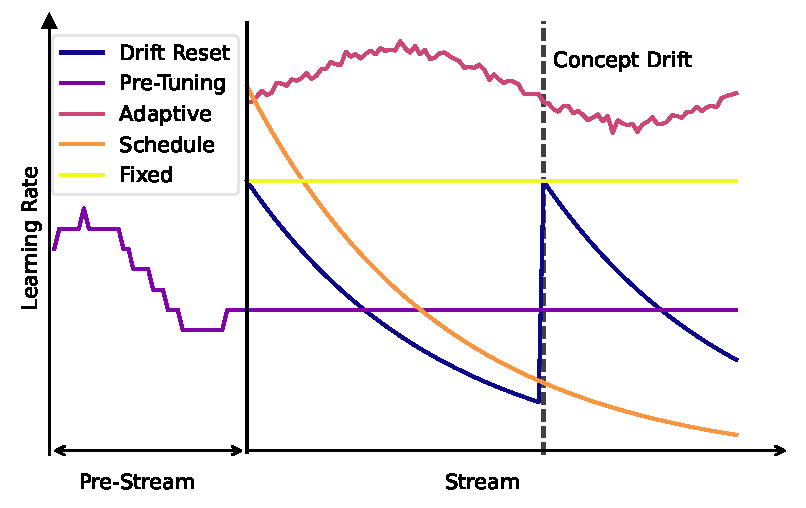
\includegraphics[width=0.8\textwidth]{figures/lr_overview.pdf}
   \caption{Overview of different learning rate optimization approaches.}
   \label{fig:lr_overview}
\end{figure}
According to \citet{bifetMOAMassiveOnline2010}, a machine learning model operating on a data stream must be able to
\begin{enumerate}
   \item[R1:] process a single instance at a time,\label{rq:single_instance}
   \item[R2:] process each instance in a limited amount of time,\label{rq:limited_time}
   \item[R3:] use a limited amount of memory,\label{rq:limited_memory}
   \item[R4:] predict at any time,\label{rq:predict_any_time}
   \item[R5:] adapt to changes in the data distribution.\label{rq:adapt_to_drift}
\end{enumerate}

These requirements pose additional challenges in selecting an appropriate optimizer and learning rate, which we describe in Section~\ref{sec:lr_in_online_learning}.
To enable more informed decisions when dealing with these challenges, we make the following contributions:

Firstly, we empirically evaluate typical learning rate schedules on a variety of synthetic and real-world data streams with different types of non-stationarities.
In this context, we also introduce and investigate the effectiveness of a mechanism that temporarily increases the learning rate upon the detection of a distributional change (i).

Secondly, within the same stream-based online learing setting, we evaluate adaptive optimization techniques that are commonly used in conventional training of neural networks and provide suggestions when to use which technique (ii).

Finally, a learning rate tuning approach adapted to stream-based learning, which we empirically show to make more effective use of any data that may be available before the online learning process (see \textit{Pre-Stream} in Figure~\ref{fig:lr_overview}) compared to conventional tuning (iii).

\section{Learning Rate in First-Order Optimization}

In the following, we will explain the theoretical background of the learning rate hyperparameter in first-order stochastic optimization.
First-order stochastic optimization algorithms, such as stochastic gradient descent, typically aim to solve the following problem
\begin{equation}
   \min_{\vtheta} \E_{\vx \sim \ptrain} [L(f(\vx; \vtheta), y)],
\end{equation}
where $L$ is a loss function that quantifies the prediction error of the model given model parameters $\vtheta$, data samples $\vx$ and their corresponding target outputs $y$, both sampled from the distribution $\ptrain$ defined by a set of training data.
The blueprint process for solving this problem using first-order stochastic optimization consists of the following steps for each iteration $t \in 0, \ldots, T$:
\begin{enumerate}
   \item Draw a mini-batch of samples $\vx_t$ from the distribution $p(\vx)$.
   \item Compute the loss $L_t = L(f(\vx_t; \vtheta_t), y_t)$ for examples $\vx_t$, labels $y_t$\footnotemark[1] and current parameters $\vtheta_t$.
   \item Compute gradient $\vg_t = \nabla_{\vtheta_t} L_t$ with respect to the parameters.
   \item Update the parameters for the next iteration using $\vg_t$ and possibly information from previous iterations.
\end{enumerate}

\footnotetext[1]{Note that for ease of notation, we denote $\vx_t$ and $y_t$ as vectors and scalars even if they are typically mini-batches of multiple examples.}

For basic SGD, we can define the parameter update performed at the end of each iteration as
\begin{equation}\label{eq:sgd_update}
   \vtheta_{t+1}  = \vtheta_{t} - \eta_t \cdot \vg_t,
\end{equation}
where $\eta_t$ denotes the step size or \textit{learning rate} at timestep $t$.

The primary trade-off concerning $\eta$ is that increasing it speeds up convergence but increases stochasticity and the risk of divergence~\citep{bengioPracticalRecommendationsGradientbased2012}.
In fact, \citet{smithBayesianPerspectiveGeneralization2018}, found that the “noise scale” of SGD is tied to $\eta$~\citep{smithBayesianPerspectiveGeneralization2018}.

\subsection{Learning Rate Schedules}

Often, the performance of a model can be improved by using a schedule that changes the learning rate as training progresses, yielding a vector of step sizes $\bm{\eta}$ that defines a step size $\eta_t$ for each timestep $t \in \{0, \ldots, T\}$~\citep{wuDemystifyingLearningRate2019b}.
For example, to ensure fast convergence early in training while mitigating jumping around potential minima later, it is common to use a decaying schedule that starts with a large learning rate and decreases over time.
An additional benefit of this approach is potentially better generalization since larger learning rates can help skip sharp minima with poor generalization~\citep{hochreiterFlatMinima1997,chaudhariEntropySGDBiasingGradient2017}.

Commonly used forms of decay are exponential decay, where $\eta_{t}$ is calculated as
$\eta_{t} = \eta_1 \cdot \gamma^t$,
with $\gamma < 1$, and stepwise decay, which for a regular interval between steps of length $s$ is given as $\eta_1 \cdot \gamma^{\lfloor t/s \rfloor}$.
Another common approach is to decay $\eta$ each time the training loss plateaus for a given number of iterations. Other popular schedules include cyclic learning rates that let $\eta$ oscillate between two values over a predefined interval.
For a triangular cycle, the learning rate is defined as
\begin{equation}
   \eta_t = \eta_1 + \frac{\hat{\eta} - \eta_1}{2s} \cdot \min_{i} \{|t-i\cdot s|\},
\end{equation}
where $\hat{\eta}$ is the learning rate at the midpoint of each cycle of length $s$.
Some studies~\citep{smithCyclicalLearningRates2017, smithSuperConvergenceVeryFast2018a} have found that cyclic schedules can significantly speed up the convergence of neural networks, in some cases even compared to adaptive techniques like Adam~\citep{kingmaAdamMethodStochastic2017b}.
While there are many alternatives, we focus on exponential, step, and cyclic learning rates as some of the most commonly used generic schedules.
For a comprehensive overview and detailed analysis of learning rate policies, see \citet{wuDemystifyingLearningRate2019b}.

\subsection{Adaptive Learning Rates}

Several studies have proposed adaptive optimizers that increase the robustness of the training process with respect to the learning rate.
These optimizers adjust the step size based on previous gradients at each step~\citep{duchiAdaptiveSubgradientMethods2011}.

One of the earlier techniques in this category is \textit{AdaGrad}~\citep{duchiAdaptiveSubgradientMethods2011}, which scales the learning rate based on the sum of squares of past gradients for each parameter, resulting in a parameter-specific step size.
Several other approaches, such as \textit{AdaDelta}~\citep{zeilerADADELTAAdaptiveLearning2012a} and \textit{RMSProp}, later built on AdaGrad's scaling approach.
The same is true for the widely used \textit{Adam} optimizer~\citep{kingmaAdamMethodStochastic2017b}, which adds a momentum term from prior gradients to speed up convergence for parameters with consistent derivatives.
Another AdaGrad-based optimizer is \textit{WNGrad}~\citep{wuWNGradLearnLearning2020}, which adaptively scales each parameter update based on the squared sum of past gradients.

So-called \textit{parameter-free} gradient-based optimization approaches aim to eliminate the learning rate completely by optimizing it as training progresses.
For example, the \textit{COCOB} algorithm~\citep{orabonaTrainingDeepNetworks2017} models parameter optimization as a gambling problem, where the goal is to maximize the reward from betting on each gradient.
The resulting strategy is equivalent to running a meta-optimization algorithm that estimates the expected optimal learning rate~\citep{orabonaTrainingDeepNetworks2017}.
Several other studies~\citep{schraudolphLocalGainAdaptation1999,vanervenMetaGradMultipleLearning2016a,baydinOnlineLearningRate2018,cutkoskyMechanicLearningRate2023} have also used the idea of learning $\eta$ via a meta-optimization process.
The \textit{hypergradient descent} (HD) approach~\citep{baydinOnlineLearningRate2018}, for example, adapts the learning rate of a base optimizer like SGD using a meta-gradient descent procedure.
However, this does not remove the learning rate entirely but replaces it with a less sensitive hypergradient step size.
\textit{Mechanic}~\citep{cutkoskyMechanicLearningRate2023} pursues the same goal by applying a meta \textit{online convex optimization} (OCO) algorithm to an arbitrary base optimizer, while \textit{stochastic meta-descent} (SMD) by \citet{schraudolphLocalGainAdaptation1999}, which extends \citeauthor{suttonAdaptingBiasGradient1992}'s work on linear systems \citep{suttonAdaptingBiasGradient1992}, uses second-order information for local adaptations of the learning rate.

\begin{table}[hb]
   \centering
   \small
   \caption{
      Overview of additional time- and space-complexity of evaluated adaptive first-order optimizers compared to basic SGD.
      Values are given in big O notation with respect to the number of model parameters $d$.
   }\label{tab:param_free_optims}
   \begin{tabular}{@{}lllcc@{}}
      \toprule
      Optimizer                & Runtime            & Space             & Param. specific & LR free \\ \midrule
      AdaGrad                  & $\mathcal{O}(5d)$  & $\mathcal{O}(1d)$ & \cmark          & \xmark  \\
      Adam                     & $\mathcal{O}(12d)$ & $\mathcal{O}(2d)$ & \cmark          & \xmark  \\
      WNGrad                   & $\mathcal{O}(2d)$  & $\mathcal{O}(0)$  & \xmark          & \xmark  \\
      COCOB                    & $\mathcal{O}(14d)$ & $\mathcal{O}(4d)$ & \cmark          & \cmark  \\
      HD\footnotemark[2]       & $\mathcal{O}(2d)$  & $\mathcal{O}(1d)$ & \xmark          & \xmark  \\
      Mechanic\footnotemark[2] & $\mathcal{O}(10d)$ & $\mathcal{O}(1d)$ & \cmark          & \cmark  \\
      DoG                      & $\mathcal{O}(5d)$  & $\mathcal{O}(1d)$ & \xmark          & \cmark  \\
      D-Adapt\footnotemark[2]  & $\mathcal{O}(6d)$  & $\mathcal{O}(2d)$ & \xmark          & \cmark  \\
      \bottomrule
   \end{tabular}
\end{table}
\footnotetext[2]{Variant with SGD as the underlying optimizer.}

Research has shown that in an OCO setting with stationary data, the worst-case optimal fixed step size for SGD is
\begin{equation}\label{eq:oco_optimal_lr}
   \eta^* = \frac{||\vtheta_1 - \vtheta^*||}{\sqrt{\sum_{t=1}^{n} ||\vg_t||^2}}.
\end{equation}
Multiple parameter-free optimizers make use of this notion.
As its name suggests, the \textit{Distance over Gradients} (DoG)~\citep{ivgiDoGSGDBest2023} algorithm estimates the unknown numerator in \Eqref{eq:oco_optimal_lr} as the maximum distance $\max_{i<t}||\vtheta_1 - \vtheta_i||$ between the initial parameters and the parameters of all previous iterations.
DoG additionally uses polynomial decay averaging as proposed by~\citet{shamirStochasticGradientDescent2012}.
\textit{D-Adaptation} by \citet{defazioLearningRateFreeLearningDAdaptation2023a}, on the other hand, employs weighted dual averaging~\citep{duchiDualAveragingDistributed2012} to compute bounds on the distance between initial and optimal parameters.

Although adaptive optimization techniques seem intuitively well suited for non-stationary data, their application to data streams has yet to be investigated.
Therefore, we assess the suitability of some of the most prominent adaptive optimizers, listed in Table~\ref{tab:param_free_optims}, for stream-based learning.

\section{Learning Rate in Online Learning}\label{sec:lr_in_online_learning}

Optimizing the learning rate in a batch learning setting involves minimizing the expected loss on a hold-out validation data set.
Formally, we can express this task as
\begin{equation}
   \label{eq:batch_lr_optim}
   \min_{\bm{\eta}} \E_{(\vx, y) \sim \hat{p}_{\rm{val}}} L(f(\vx; \vtheta_n), y),
\end{equation}
where samples $(\vx, y)$ are drawn from a distribution $\hat{p}_{\rm{val}}$ defined by a validation dataset and $\vtheta_n$ are the model parameters at the end of training that depend on the learning rate schedule $\bm{\eta}$.
In online learning, where data is generated incrementally, this notion of learning rate optimization is not feasible.
Due to requirements \textbf{R1-R5}, models operating in an online learning environment should be evaluated in a \textit{prequential} manner~\citep{bifetMOAMassiveOnline2010}, where each sample $\vx_t$ in the data stream is first used to test and then to train the model, ensuring that testing is done on previously unobserved data.

Training in such a scenario can be more accurately modeled as an online convex optimization problem~\citep{shalev-shwartzOnlineLearningOnline2011,hazanIntroductionOnlineConvex2016}, where the optimizer suffers a loss $L(f(\vx; \vtheta_t), y)$ and produces updated parameters $\vtheta_{t+1}$ at each iteration of the data stream.
Learning rate optimization in this setting can be formulated as
\begin{equation}
   \label{eq:stream_lr_optim}
   \min_{\bm{\eta}} \sum_{t=1}^{n} \E_{(\vx, y) \sim \hat{p}_{\rm{stream}}^{(t)}} L(f(\vx; \vtheta_t), y).
\end{equation}

Compared to \Eqref{eq:batch_lr_optim}, \Eqref{eq:stream_lr_optim} features some key differences.
Due to the requirement to be able to predict at any time (\textbf{R4}), the goal is to minimize the expected total sum of losses over all timesteps of the prequential evaluation process instead of the validation loss for the final parameters $\vtheta_n$.
Therefore, the speed of convergence is more critical in the streaming setting, while the performance of the final $\vtheta_n$ parameter has a much smaller impact.
Since memory is limited (Requirement~\ref{rq:limited_memory}), it is also impossible to continue training on previously observed data as long as the loss decreases, putting even more emphasis on fast adaptation.
At the same time, a higher learning rate that temporarily increases the loss by skipping local minima may be suboptimal with respect to \Eqref{eq:stream_lr_optim}, even if it eventually leads to a lower loss.
Another difference to conventional batch learning is that the data distribution $\hat{p}_{\rm{stream}}^{(t)}$ is time-dependent because streams are often subject to distributional changes such as \textit{concept drifts} over time \citep{widmerLearningPresenceConcept1996}.
While other forms of drifts exist, we use \textit{concept drift} as an umbrella term for any kind of distributional shift in the following.

\subsection{Learning Rate Tuning}\label{subsec:pre-tuning}

Although strict online learning assumes that no data is available prior to the deployment of a model in the streaming environment, limited amounts of data may be available prior to the stream learning process in many real-world applications.
Such data can then be used to tune the learning rate of the model before stream deployment (pre-stream).
However, the differences in evaluation schemes described above may cause conventional learning rate tuning to produce poor results for stream-based learning.
In offline learning, learning rate tuning is typically performed by repeating the training process for a grid of possible parameter values and selecting the value that yields the best target metric on a held-out validation set after the training is completed.
As a result of only considering the performance at the end and not throughout the training process, this tuning approach may result in poor results with respect to the goal of learning rate optimization in streaming environments (see \Eqref{eq:stream_lr_optim}).
Therefore, we propose the modified tuning approach described in \Cref{alg:pre-tuning} aimed at approximating \Eqref{eq:stream_lr_optim}, which we call learning rate \textit{pre-tuning}.

\begin{algorithm}[t]
   \caption{Pre-Stream Learning Rate Tuning for Online Learning Models}\label{alg:pre-tuning}
   \begin{algorithmic}[1]
      \Require Set of learning rate values $\sH$, set of schedule parameter values $\sG$, data samples $\sX$
      \Require Optimization function $o$, metric function to tune $m$, number of tuning steps $n_{\rm{steps}}$

      \State $\sS \gets \{(\vx_i, y_i) \sim \hat{p}_{\sX}| \forall i \in \{1, \ldots, n_{\text{steps}}\} \}$ \Comment{Create artificial stream by sampling $\sX$ with replacement.}
      \State $v^* \gets -\infty$
      \For{$\eta$ \textbf{in} $\sH$, $\gamma$ \textbf{in} $\sG$}
      \State $v \gets v_{\textrm{init}}$ \Comment{Initialize metric value.}
      \For{$\vx, y$ \textbf{in} $\sS$}
      \State $\hat{y} \gets f(\vx, \vtheta)$ \Comment{Calculate predictions with model function $f$.}
      \State $v \gets m(\hat{y}, y, v)$ \Comment{Update metric value.}
      \State $\vg \gets \nabla_{\vtheta} L(\hat{y}, y)$ \Comment{Calculate gradient of predictive loss w.r.t. $\vtheta$.}
      \State $\vtheta, \eta \gets o(\vtheta, \vg, \eta, \gamma)$ \Comment{Update model parameters $\vtheta$ and learning rate $\eta$.}
      \EndFor
      \If{$v > v^*$}
      \State $\eta^* \gets \eta$ \Comment{Update best learning rate.}
      \State $\gamma^* \gets \gamma$ \Comment{Update best schedule parameters.}
      \EndIf
      \EndFor
      \State \textbf{return} $\eta^*, \gamma^*$ \Comment{Return best hyperparameter values.}
   \end{algorithmic}
\end{algorithm}

To emulate the data stream to be processed after tuning, we continuously draw samples with replacement from the tuning data $\sX$ in a bootstrapping procedure instead of training on all data for multiple epochs.
By doing so, we aim to increase the variability of the data and, thus, the similarity to a real data stream.
We then optimize the learning rate and any optional learning rate schedule parameters $\gamma$ with respect to the selected performance metric $m$ over the emulated stream $\sS$.
While we use a simple grid search in \cref{alg:pre-tuning}, any parameter search technique could be used for this purpose.
We provide a detailed experimental evaluation of our approach in Section~\ref{sec:experiments}.

\subsection{Concept Drift Adaptation}

Concept drift requires repeated adaptation of the model parameters.
If post-drift training is interpreted as a new online optimization problem, the worst-case optimal learning rate can be computed according to \Eqref{eq:oco_optimal_lr}, replacing the initial parameter values $\vtheta_1$ with the values at the time of drift onset $\vtheta_{t_{\rm{drift}}}$.
As a result, stronger drifts that cause $\vtheta^*$ to move away from $\vtheta_{t_{\rm{drift}}}$ can benefit from larger learning rates.

Based on this notion, we propose a simple adaptation to decaying learning rate schedules that resets $\eta$ to its original value when a concept drift is detected.
An exponential schedule modified with our approach will thus yield learning rates of
\begin{equation}
   \eta_t = \eta_1 \cdot \gamma^{t-t_{\rm{drift}}},
\end{equation}\label{eq:drift_reset}
where $t_{\rm{drift}}$ marks the timestep at which the drift was last detected.
For drift detection, we apply either \textit{ADWIN}~\citep{bifetLearningTimeChangingData2007} or the Kolmogorov-Smirnov test~\citep{masseyKolmogorovSmirnovTestGoodness1951} to the prequential losses.
To avoid detecting loss decreases as concept drifts, we test only for increases of the prequential loss.

Our approach is similar to forgetting mechanisms commonly used in conventional online learning~\citep{gamaSurveyConceptDrift2014}.
To improve model plasticity, such mechanisms reset the current model parameters to their initial values.
While the simplest implementation of forgetting resets all parameters, there is a variety of more targeted approaches for increasing model plasticity.
For instance, \citet{dohareLossPlasticityDeep2023} suggest computing a utility metric and resetting neurons that receive a low utility value, while \citet{paikOvercomingCatastrophicForgetting2019a} instead adapt the learning rate for each neuron using a utility metric.
Similarly, \citet{elsayedUtilitybasedPerturbedGradient2023} limits changes to high-utility-weights while intentionally perturbing low-utility-weights.


\section{Experiments}\label{sec:experiments}

We empirically evaluate our hypotheses using the following setup\footnote[3]{Code available at \url{https://github.com/lucasczz/OLRONN}.}:

We use synthetic and publicly available real-world classification datasets with different sizes and types of concept drift, listed in Table~\ref{tab:datasets}.
Our evaluations include the \textit{Agrawal} stream-generator~\citep{agrawalDatabaseMiningPerformance1993} for which we introduce concept drift by gradually switching the function that defines the target variable between the 45,000th and the 55,000th sample.
We also use the \textit{LED} generator~\citep{gordonClassificationRegressionTrees1984}, switching 5 of the 7 relevant features with irrelevant ones between instances 25000 and 75000.
For the \textit{Random Radial Basis Function} (RBF) datasets, we incorporate abrupt (RBF\textsubscript{a}) or incremental (RBF\textsubscript{i}) concept drift by switching or moving the centroids of the data distribution.
We further employ the \textit{Electricity} and \textit{Covertype}~\citep{misc_covertype_31} datasets, which are commonly used to evaluate online learning models, as well as two \textit{Insects} datasets~\citep{souzaChallengesBenchmarkingStream2020} with predefined types of concept drift.
In the following sections, we exclude the results for the RBF\textsubscript{i} and Insects\textsubscript{i} datasets, which can instead be found in \Cref{app:full_results}.

With respect to the neural network architecture, we limit our investigations to multi-layer perceptrons (MLPs) with a single-hidden-layer and hidden units matching the number of input features implemented with \textit{PyTorch}~\citep{paszkePyTorchImperativeStyle2019}.
Even though more elaborate architectures could, in theory, produce better results, they also typically require more tuning and longer training than smaller models, making them less suited for streaming environments.

We tune the base learning rate $\eta_1$ of all but the parameter-free approaches using a grid search of ten geometrically spaced values and configure adaptive optimizers with their default parameter values. For HD, Mechanic, and D-Adaptation, we select SGD as the base algorithm.
We select a fixed factor $\gamma$ for decay schedules on all datasets based on what we found to perform well across several scenarios in our preliminary investigations.
For the proposed learning rate resetting mechanism, we select a smaller decay factor and set the confidence level $\delta$ for drift detection to $10^{-4}$.
For our evaluations, we process each dataset sequentially, emulating streams of mini-batches of four instances each while recording the prequential accuracy and other metrics in intervals of 25 iterations.
We refer to \Cref{app:hyperparams} for more detailed information on our experimental setup.
We report our results as averages over five random seeds.

\begin{table}[hb]
   \centering
   \small
   \caption{Datasets used for experimental evaluations.}
   \begin{tabular}{@{}clcccc@{}}
      \toprule
      Type                    & Data Stream              & Instances               & Features & Classes \\
      \midrule
      \multirow{4}{*}{Synth.} & Agrawal                  & 100,000                 & 9        & 2       \\
                              & LED                      & 100,000                 & 24       & 10      \\
                              & RBF\textsubscript{a}     & 100,000                 & 20       & 5       \\
                              & RBF\textsubscript{i}     & 100,000                 & 20       & 5       \\
      \midrule
      \multirow{5}{*}{Real}   & Covertype                & 100,000\footnotemark[4] & 54       & 7       \\
                              & Electricity              & 45,312                  & 8        & 2       \\
                              & Insects\textsubscript{a} & 52,848                  & 33       & 6       \\
                              & Insects\textsubscript{g} & 24,150                  & 33       & 6       \\
                              & Insects\textsubscript{i} & 57,018                  & 33       & 6       \\
      \bottomrule
   \end{tabular}
   \label{tab:datasets}
\end{table}

\footnotetext[4]{For Covertype we use only the first 100,000 from a total of 581,012 instances.}


\subsection{Learning Rate Schedules}

To evaluate the effectiveness of our learning rate resetting mechanism for drift adaptation (see \Eqref{eq:drift_reset}), we compare its average prequential accuracy to that of model weight resetting and non-adaptive learning rate schedules, commonly used in online learning.

As seen in Table~\ref{tab:lr_resetting}, our approach outperforms weight-resetting on all but Covertype but rarely yields an advantage over a basic exponential or fixed learning rate.
Since both variants of our resetting approach perform almost identically, this performance gap is likely not caused by the drift detector.
Instead, it appears that most concept drifts, even artificially created ones, are not severe enough for a drastic learning rate increase to be beneficial compared to the better stability of a more continuous learning rate progression.


\begin{table}[ht]
   \centering
   \small
   \caption{Average prequential accuracy [\%] for static and drift adaptive learning rate schedules with SGD. LR-Reset\textsubscript{A} uses ADWIN, LR-Reset\textsubscript{K} uses Kolmogorov-Smirnov testing for drift detection. Best values are shown in \textbf{bold}, values within the $1\sigma$ interval of best values \underline{underlined}.}
   \begin{tabular}{llllllll}
      \toprule
      Schedule                  & Agrawal                    & LED                      & RBF\textsubscript{a}       & Covertype                  & Electricity                & Insects\textsubscript{a}   & Insects\textsubscript{g}   \\
      \midrule

      Fixed                     & \bfseries 79.78$\pm$1.09   & \bfseries 73.91$\pm$0.04 & \bfseries 89.57$\pm$2.61   & \underline{83.42$\pm$0.50} & \bfseries 73.77$\pm$0.40   & 71.50$\pm$0.08             & 75.31$\pm$0.21             \\
      Exp.                      & 77.98$\pm$1.36             & 73.38$\pm$0.14           & \underline{87.66$\pm$3.53} & 82.95$\pm$0.26             & \underline{73.51$\pm$0.48} & \underline{72.19$\pm$0.37} & \bfseries 75.91$\pm$0.14   \\
      Step                      & 76.56$\pm$1.13             & 72.86$\pm$0.18           & 84.98$\pm$6.46             & 82.89$\pm$0.37             & \underline{73.62$\pm$0.53} & \bfseries 72.23$\pm$0.27   & \underline{75.83$\pm$0.21} \\
      Cyclic                    & \underline{78.72$\pm$0.90} & 73.67$\pm$0.17           & \underline{88.40$\pm$4.26} & \bfseries 83.44$\pm$0.08   & 68.38$\pm$0.81             & 71.74$\pm$0.39             & 75.64$\pm$0.06             \\
      Weight-Reset              & 72.03$\pm$0.91             & 64.31$\pm$2.16           & 70.41$\pm$0.92             & 82.92$\pm$0.57             & 71.17$\pm$0.62             & 63.55$\pm$0.42             & 69.66$\pm$0.65             \\
      LR-Reset\textsubscript{A} & 78.26$\pm$0.73             & 72.95$\pm$0.13           & \underline{87.60$\pm$3.43} & 82.92$\pm$0.32             & 73.07$\pm$0.66             & 71.48$\pm$0.34             & 75.54$\pm$0.11             \\
      LR-Reset\textsubscript{K} & 78.27$\pm$1.88             & 72.95$\pm$0.13           & \underline{87.60$\pm$3.43} & 82.92$\pm$0.32             & 73.07$\pm$0.66             & 71.48$\pm$0.34             & 75.54$\pm$0.11             \\
      \bottomrule
   \end{tabular}
   \label{tab:lr_resetting}
\end{table}

\def\asize{0.5\textwidth}
\begin{figure}[ht]
   \centering
   \begin{subfigure}[b]{\asize}
      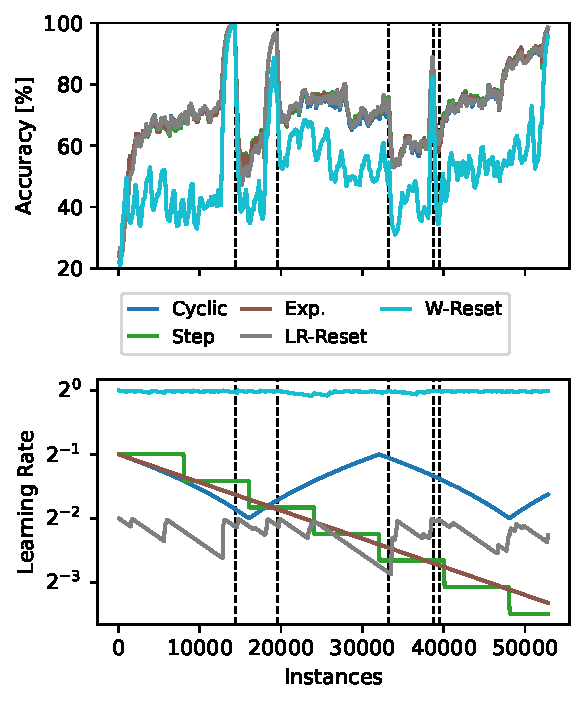
\includegraphics[width=\textwidth]{figures/lr_norms_schedules_insects_abrupt.pdf}
      \caption{Schedules}
      \label{fig:prequential_schedulers_insects}
   \end{subfigure}
   \begin{subfigure}[b]{0.99\textwidth - \asize}
      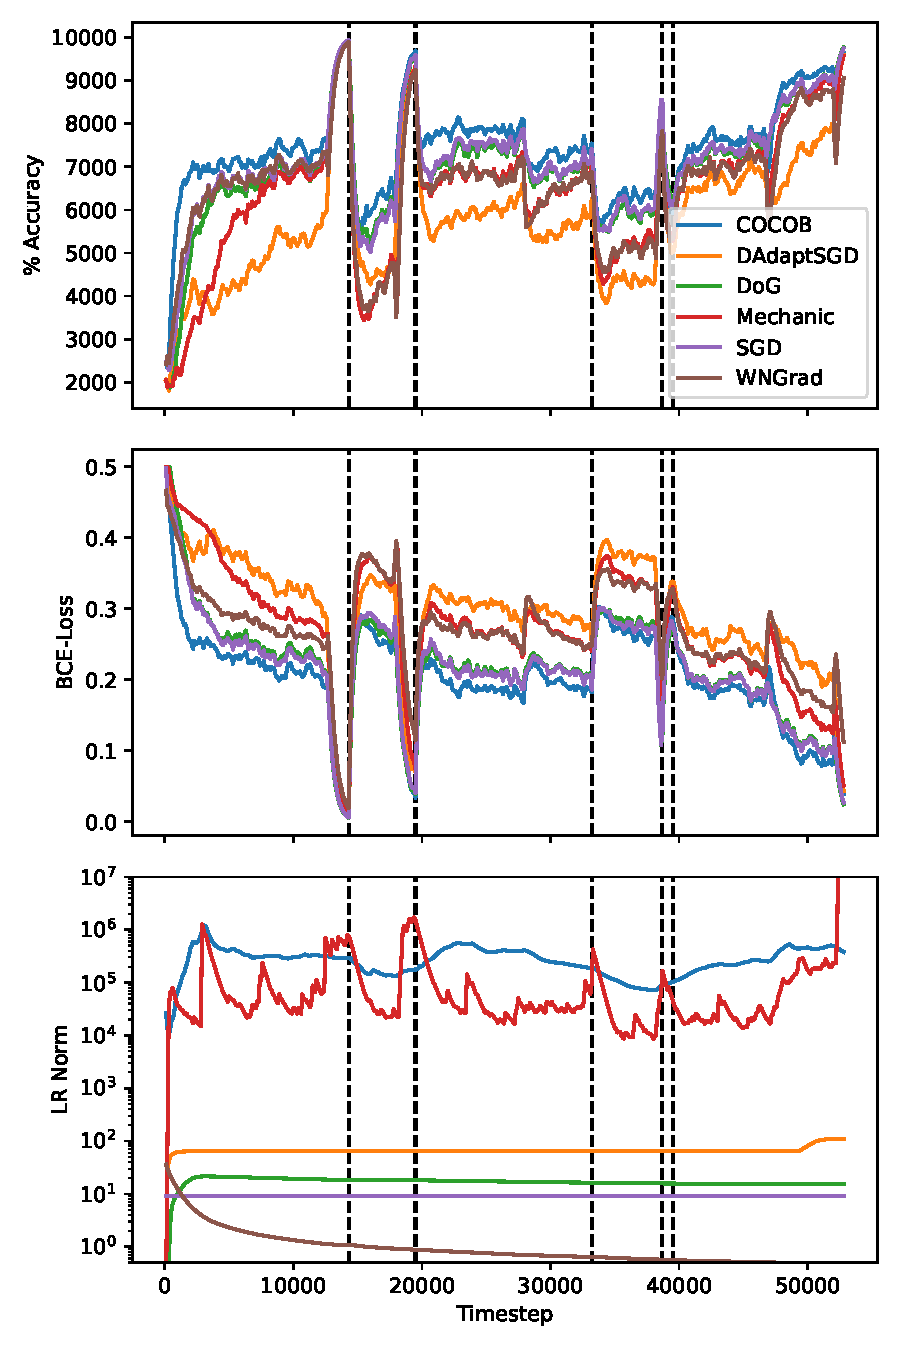
\includegraphics[width=\textwidth]{figures/lr_norms_optims_insects_abrupt.pdf}
      \caption{Adaptive Optimizers}
      \label{fig:prequential_optims_insects}
   \end{subfigure}
   \caption{Prequential accuracy and learning rate for different schedules and adaptive optimizers on Insects\textsubscript{a} dataset. Concept drifts are marked by dashed lines. Accuracy is exponentially smoothed with a decay factor of 0.75. Note that the learning rates of COCOB, Adam, and Mechanic in \ref{sub@fig:prequential_optims_insects} are much larger compared to DoG etc. due to being scaled by an estimate of the second-moment of past gradients.}
\end{figure}

With accuracy values within $1\sigma$ of each other on all evaluated streams, the stepwise decay shows almost identical performance to the exponential decay.
The accuracy of the cyclic schedule for Covertype slightly surpasses the one achieved with a fixed learning rate but lags behind on most real-world streams.
We also did not find an order of magnitude improvement in convergence speed as observed by~\citep{smithSuperConvergenceVeryFast2018a} for the scenario studied.

Despite the intuition, that increasing the learning rate on concept-drifts should increase the average performance, our experiments suggest, that an appropriate fixed learning rate is preferable to both drift-adaptive as well as static schedules for most online learing scenarios.

\subsection{Adaptive Learning Rates}

Our results for adaptive optimizers displayed in Table~\ref{tab:results_adaptive_optims}, show a strong data dependency as none of the evaluated algorithms consistently outperforms its competitors.
However, since SGD yields a high average accuracy on RBF\textsubscript{a} but is clearly surpassed on Insects\textsubscript{a}, the type of concept drift does not seem to be significant.
Due to its favorable performance in terms of average accuracy and computational efficiency, SGD should be selected out of the non-parameter-free approaches in most cases.
While some of the more elaborate optimizers like Adam or the SGD variant of Hypergradient Descent (HD)~\citep{baydinOnlineLearningRate2018} and WNGrad~\citep{wuWNGradLearnLearning2020} also yield high accuracy scores in our experiments, they incur a more significant computational cost compared to SGD.

\begin{table}[t]
   \centering
   \small
   \caption{Average prequential accuracy [\%] for different optimizers. Best values are shown in \textbf{bold}, values within the $1\sigma$ interval of best values \underline{underlined}.}
   \begin{tabular}{lllllllll}
      \toprule
                                                         & Optimizer & Agrawal                    & LED                       & RBF\textsubscript{a}       & Covertype                 & Electricity             & Insects\textsubscript{a} & Insects\textsubscript{g} \\
      \midrule
      \multirow{5}{*}{\rotatebox[origin=t]{90}{Tuned}}   & SGD       & \underline{79.64$\pm$2.03} & \underline{73.91$\pm$.04} & \underline{89.57$\pm$2.61} & \bfseries 83.42$\pm$.50   & 73.77$\pm$.40           & 71.50$\pm$.08            & 75.31$\pm$.21            \\
                                                         & Adam      & \underline{78.91$\pm$2.40} & \bfseries 73.98$\pm$.20   & 86.33$\pm$1.85             & 79.01$\pm$.27             & 69.79$\pm$.54           & \bfseries 75.38$\pm$.24  & 75.78$\pm$.74            \\
                                                         & AdaGrad   & \underline{79.13$\pm$1.62} & 72.55$\pm$.31             & 81.92$\pm$3.89             & 81.68$\pm$.35             & 76.99$\pm$1.20          & 74.87$\pm$.40            & 77.15$\pm$.27            \\
                                                         & WNGrad    & 76.91$\pm$.47              & 64.66$\pm$.34             & 80.07$\pm$.67              & 76.98$\pm$.15             & 70.80$\pm$.59           & 66.25$\pm$.19            & 66.75$\pm$.40            \\
                                                         & HD        & \bfseries 80.19$\pm$1.56   & 73.81$\pm$.09             & \underline{89.78$\pm$3.37} & \underline{83.36$\pm$.25} & 73.83$\pm$.32           & 70.67$\pm$.06            & 73.37$\pm$.21            \\
      \midrule
      \multirow{4}{*}{\rotatebox[origin=t]{90}{LR-Free}} & COCOB     & 78.21$\pm$1.12             & \underline{73.88$\pm$.50} & \bfseries 90.75$\pm$1.28   & 82.27$\pm$.46             & \bfseries 84.48$\pm$.88 & 74.75$\pm$.11            & \bfseries 77.67$\pm$.17  \\
                                                         & DoG       & \underline{78.77$\pm$2.25} & 73.34$\pm$.13             & 87.04$\pm$3.13             & 83.07$\pm$.64             & 71.53$\pm$.70           & 70.59$\pm$.26            & 74.01$\pm$.21            \\
                                                         & D-Adapt   & 60.16$\pm$.96              & 54.69$\pm$8.34            & 41.37$\pm$3.34             & 76.69$\pm$.79             & 66.03$\pm$1.75          & 50.05$\pm$11.26          & 48.21$\pm$10.62          \\
                                                         & Mechanic  & 62.09$\pm$9.20             & 69.04$\pm$.19             & 87.33$\pm$.50              & 78.67$\pm$.18             & 50.73$\pm$7.60          & 55.31$\pm$21.47          & 65.80$\pm$.53            \\
      \bottomrule
   \end{tabular}
   \label{tab:results_adaptive_optims}
\end{table}
In the category of learning-rate-free optimizers, COCOB~\citep{orabonaTrainingDeepNetworks2017} outperformed its competitors on all but two datasets.
It comes close to or even exceeds the best tuned approaches in terms of accuracy.
Although yielding lower accuracy on average, DoG also comes within reach of the tuned methods while offering much better runtime and memory efficiency compared to COCOB (see Table~\ref{tab:param_free_optims}).
Mechanic~\citep{cutkoskyMechanicLearningRate2023} and D-Adaptation~\citep{defazioLearningRateFreeLearningDAdaptation2023a} performed significantly worse than their competitors on the evaluated streams.

The learning rate curves shown in Figure~\ref{fig:prequential_schedulers_insects} indicate the reason for the poor performance of WNGrad and D-Adaption.
Whereas the learning rate of DoG quickly approaches the optimal learning rate, WNGrad and D-Adaptation diverge considerably from it.

The best-performing Adam's learning rate exhibits spikes for most change points, suggesting some form of adaptability to drift.
However, since the much worse performing Mechanic shows similar spikes, this is unlikely to contribute significantly to Adam's high accuracy on Insects\textsubscript{a}.
Instead, it likely stems from its second-moment scaling, also featured in the similarly performing AdaGrad.

All in all, COCOB shows the most promising results in terms of average prequential accuracy, making it preferable over the competing approaches if its larger memory- and computational footprint are permissibe.
In scearios with limited computational resources on the other hand, DoG may be a more viable choice due to its efficiency.

\subsection{Learning Rate Tuning}

We evaluate our Pre-Tuning approach by using either 500 or 1000 instances held out at the beginning of each stream for tuning. We assess Multi-Layer Perceptrons (MLPs) with 64 or 128 hidden units per layer and either one or three hidden layers.
To determine the learning rate and decay factor, we rely on the optimal mean prequential accuracy. This choice accounts for the potential bias towards learning rates associated with lower initial losses, as loss values often decrease notably during training.

Figure~\ref{fig:pretune_lr_accuracy} shows the absolute difference between the learning rate resulting from the Pre-Tuning process and the optimal value $|\eta_p - \eta^*|$ at each tuning step averaged over all real-world datasets and network architectures.

\begin{figure}[!ht]
   \centering
   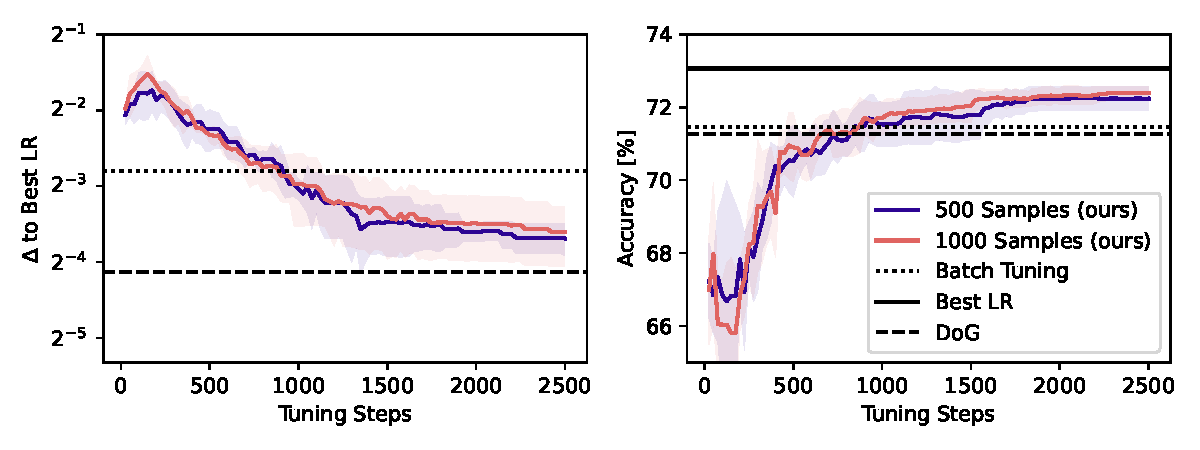
\includegraphics[width=\textwidth]{figures/pretune_all_acc_lr_exp_schedule.pdf}
   \caption{Absolute difference between pre-tuned and optimal learning rate and resulting accuracy on data streams for SGD and an exponential learning rate schedule with 500 or 1000 tuning samples. DoG is not included in first subplot since it is not intended for use with LR decay. Results are averaged over all real-world datasets and network architectures. The shaded area represents the 1$\sigma$-interval.}\label{fig:pretune_lr_accuracy}
\end{figure}
\begin{table}[!hb]
   \centering
   \small
   \caption{
      Prequential accuracy of learning rate tuning approaches averaged over all investigated MLP architectures. For Pre-Tuning\textsubscript{500} and Pre-Tuning\textsubscript{1000} we run our proposed learning rate tuning approach for 2000 steps with either 500 or 1000 samples and select the learning rate yielding the highest average prequential accuracy over the tuning run.
   }\label{tab:lr_tuning}
   \begin{tabular}{lllllllllll}
      \toprule
      Approach                       & Agrawal                 & LED                     & RBF\textsubscript{a}    & Covertype                 & Electricity               & Insects\textsubscript{a} & Insects\textsubscript{g}  \\
      \midrule
      SGD (Best LR)                  & 83.70                   & 73.95                   & 93.84                   & 83.14                     & 74.15                     & 71.98                    & 75.28                     \\
      COCOB                          & 83.71$\pm$.25           & 74.34$\pm$.09           & 95.29$\pm$.24           & 82.96$\pm$.19             & 84.57$\pm$.08             & 75.39$\pm$.10            & 77.62$\pm$.08             \\ \midrule
      DoG                            & 82.06$\pm$.52           & \bfseries 73.71$\pm$.11 & 91.36$\pm$.46           & \bfseries 82.56$\pm$.15   & 70.47$\pm$.40             & 70.59$\pm$.10            & 73.92$\pm$.11             \\
      Batch Tuning                   & 81.09$\pm$1.34          & 66.67$\pm$3.28          & 91.89$\pm$.39           & 82.41$\pm$.61             & 72.86$\pm$.76             & 69.81$\pm$2.18           & 73.91$\pm$.64             \\
      Pre-Tuning\textsubscript{500}  & 82.01$\pm$.32           & 73.26$\pm$.03           & \bfseries 92.36$\pm$.03 & \underline{82.42$\pm$.07} & \underline{73.34$\pm$.45} & \bfseries 71.81$\pm$.04  & \bfseries 75.22$\pm$.08   \\
      Pre-Tuning\textsubscript{1000} & \bfseries 82.56$\pm$.25 & 73.30$\pm$.00           & 92.18$\pm$.38           & \underline{82.47$\pm$.18} & \bfseries 73.37$\pm$.34   & \bfseries 71.81$\pm$.06  & \underline{75.17$\pm$.05} \\
      \bottomrule
   \end{tabular}
\end{table}

Batch tuning with 800 training and 200 validation samples initially yields a better approximation of the optimal learning rate. However, our streaming-specific approach undercuts the baseline after 1000 tuning steps, consistently decreasing and ultimately reaching approximately half of the approximation error observed in batch tuning.
The performance also remains nearly identical, even when using only 500 samples for tuning, demonstrating the data efficiency of Pre-Tuning.

The superior performance of our approach is also reflected in the accuracy scores depicted in the right subfigure of Figure~\ref{fig:pretune_lr_accuracy}.
In fewer than 1000 steps, our approach comes closer to the optimal learning rate and also exceeds the accuracy of conventional tuning.
Notably, our approach's usage of the average prequential accuracy more accurately resembles the online learning process and sets it apart from conventional tuning, which solely focuses on performance at the end of the tuning process.
Pre-Tuning also surpasses DoG, which we selected as a baseline due to being the best-performing parameter-free technique within the group of optimizers with a global learning rate that is the most comparable to our approach.
This advantage comes despite a smaller average absolute deviation of DoG compared to our approach, which can be explained by the fact that DoG strongly underestimates the optimal learning rate at the beginning of training (see e.g. \Cref{sub@fig:prequential_optims_insects}), where fast adaptation is crucial.
Because DoG closely approaches the best learning rate for most of the stream, this barely affects its average deviation from the optimal learning rate.

The effectiveness of Pre-Tuning can also be seen in the dataset-specific results displayed in \Cref{tab:lr_tuning}.
Our tuning technique executed with 1000 samples (Pre-Tuning\textsubscript{1000}) outperforms DoG and conventional tuning on all but the LED and Covertype datasets and often approaches the best learning rate determined via tuning directly on the testing stream (SGD Best LR).
Even with 500 samples, the technique yields favorable results, indicating its usefulness in cases where data that is available pre-stream is scarce.
While much more computationally expensive than the other evaluated approaches, the COCOB optimizer provides much better accuracy scores across all investigated data streams.

In conclusion, our proposed tuning approach enables significantly better learning rate selection for prequential evaluation on data streams than conventional tuning and DoG.
Compared to learning-rate-free approaches like DoG or COCOB, Pre-Tuning also has the benefit that no additional memory or runtime costs are incurred once completed.
This could be a critical advantage in streaming applications, where computing resources are often times a limiting factor.
However, if computational efficiency is insignificant, the highly performant but expensive COCOB~\citep{orabonaTrainingDeepNetworks2017} or the slightly less performant and much less expensive DoG~\citep{ivgiDoGSGDBest2023} may be more appropriate.
The usefulness of our Pre-Tuning approach is also likely limited in cases where the available tuning data is not representative of the subsequent data stream, such as for data streams with extreme concept drift.
In such cases, approaches with a dynamic learning rate are presumably superior.

\section{Conclusion}

In this work, we investigate the influence and selection of the learning rate and optimization procedure with respect to training neural networks in streaming environments.
First, we provide a theoretical background on the differences between learning rate optimization in conventional batch learning and online learning.

Based on these differences, we propose a simple mechanism that resets a decayed learning rate upon concept drift occurrences to increase the speed of adaptation, which we evaluate on several synthetic and real data streams.
Our evaluations show that our adaptation mechanism is much more effective when using neural networks than resetting model weights, which is commonly done in conventional online learning.
However, contrary to the intuition that temporarily increasing plasticity via the learning rate in response to concept drift should have a positive impact on the average model performance, an appropriate fixed learning rate yielded better results in most cases.

Furthermore, we experimentally compare adaptive optimization techniques popular for batch learning purposes in the context of online learning.
We find that the DoG and especially the COCOB optimizer yield high average accuracy scores even when compared to techniques that require manual step size tuning.
Based on these results, we suggest the use of COCOB in applications where its higher computational cost compared to DoG can be accommodated.

Finally, we contribute the streaming-specific \textit{pre-tuning} approach, which uses data available prior to the online learning process in a novel way, achieving significant performance gains over conventional tuning via a train-validation split, and providing another valuable alternative to the computationally expensive COCOB.

\subsubsection*{Acknowledgements}

This work was carried out with the support of the German Federal Ministry for Economic Affairs and Climate Action (BMWK) within the project "LieferBotNet" (Grant 01ME21001C) and received funding from the Energy and Climate Fund under chapter 6092, title 68304, fiscal year 2021.

\bibliography{collas2024_conference}
\bibliographystyle{collas2024_conference}

\newpage
\appendix
\section{Hyperparameter Settings for Empirical Evaluation}\label{app:hyperparams}

\begin{table}[h]
   \centering
   \caption{Variable notation as used in this work.}
   \begin{tabular}{lr}
      \toprule
      Parameter                        & Symbol       \\
      \midrule
      Model Parameters                 & $\vtheta $   \\
      Loss Function                    & $L$          \\
      Learning Rate                    & $\eta$       \\
      Learning Rate Decay Factor       & $\gamma$     \\
      Drift Detection Confidence Level & $\delta$     \\
      Steps Between LR Cycles/Updates  & $s$          \\
      Relative LR at Midpoint of Cycle & $\hat{\eta}$ \\
      \bottomrule
   \end{tabular}
\end{table}

\begin{table}[h]
   \centering
   \caption{Search spaces for learning rate of different optimizers.}
   \begin{tabular}{l l}
      \toprule
      Optimizer & Learning Rate Search Space                \\
      \midrule
      SGD       & ${2^1, 2^0, ..., 2^{-8}}$                 \\
      Adam      & ${2^{-3}, 2^{-4}, ..., 2^{-12}}$          \\
      AdaGrad   & ${2^1, 2^0, ..., 2^{-8}}$                 \\
      WNGrad    & ${10^{1.25}, 10^{0.75}, ..., 10^{-7.75}}$ \\
      HD        & ${2^{-3}, 2^{-4}, ..., 2^{-12}}$          \\
      COCOB     & $100$                                     \\
      DoG       & $1$                                       \\
      D-Adapt   & $1$                                       \\
      Mechanic  & $0.01$                                    \\
      \bottomrule
   \end{tabular}
\end{table}

\begin{table}[ht]
   \centering
   \caption{Configuration of other parameters.}
   \begin{tabular}{l l}
      \toprule
      Schedule    & Values                                  \\
      \midrule
      Exponential & $\gamma = 1 - 2^{-13}$                  \\
      LR-Reset    & $\gamma = 1 - 2^{-12}, \delta = 0.0001$ \\
      Step        & $\gamma = 0.75, s = 2000$               \\
      Cyclic      & $\hat{\eta} = 0.25, s = 8000$           \\
      \bottomrule
   \end{tabular}
\end{table}
\newpage
\section{Full Experimental Results}\label{app:full_results}

In this section, we provide our full experimental results including the RBF\textsubscript{i} and Insects\textsubscript{i} datastreams as well as a detailed

\subsection{Architecture-specific Learning Rate Tuning Results}\label{app:tuning_architectures}

\begin{figure}[h]
   \centering
   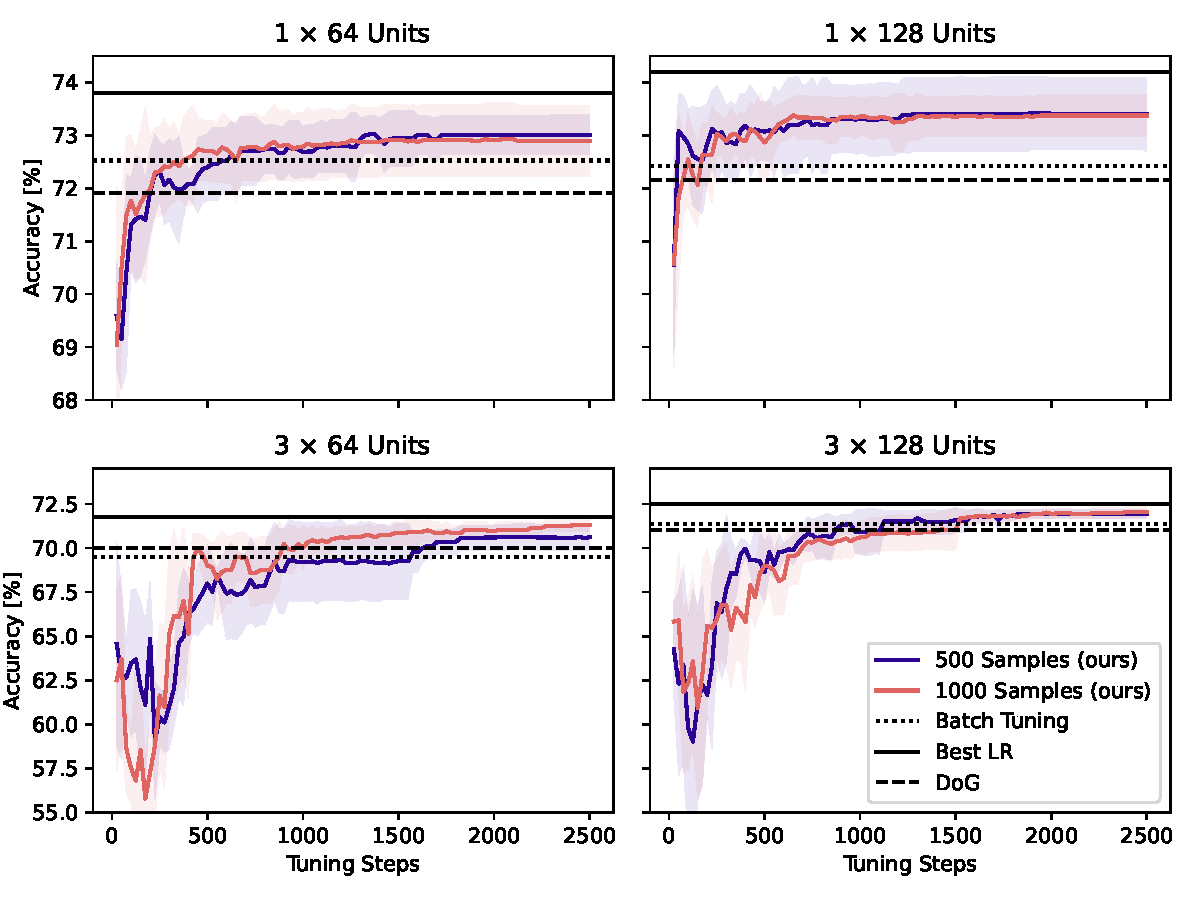
\includegraphics[width=\textwidth]{figures/pretune_architectures_exp_schedule.pdf}
   \caption{Average accuracy over all evalutated real-world datasets achieved by Pre-Tuning for different network architectures.}
\end{figure}

\newpage
\subsection{Full Results on Learning Rate Tuning}\label{app:tuning_results}
\vfill

\captionsetup{hypcap=false}

\begin{center}
   \begin{sideways}
      \begin{minipage}{0.9\textheight}
         \centering
         \scriptsize
         \captionof{table}{
            Full prequential accuracy results of learning rate tuning approaches averaged over all investigated MLP architectures. For Pre-Tuning\textsubscript{500} and Pre-Tuning\textsubscript{1000} we run our proposed learning rate tuning approach for 2000 steps with either 500 or 1000 samples and select the learning rate yielding the highest average prequential accuracy over the tuning run. In addition to the streams shown in the main body, we also evaluated a Rotated MNIST dataset consisting of four consecutive subsets of 25000 images rotated at a specific angle.
         }
         \begin{tabular}{lllllllllll}
            \toprule
            Approach                       & Agrawal                 & LED                     & RBF\textsubscript{a}    & RBF\textsubscript{i}     & Rotated MNIST             & Covertype                 & Electricity               & Insects\textsubscript{a} & Insects\textsubscript{g}  & Insects\textsubscript{i} \\
            \midrule
            SGD (Best LR)                  & 83.70                   & 73.95                   & 93.84                   & 81.52                    & 89.82                     & 83.14                     & 74.15                     & 71.98                    & 75.28                     & 60.75                    \\
            COCOB                          & 83.71$\pm$.25           & 74.34$\pm$.09           & 95.29$\pm$.24           & 78.59$\pm$.38            & 90.66$\pm$.08             & 82.96$\pm$.19             & 84.57$\pm$.08             & 75.39$\pm$.10            & 77.62$\pm$.08             & 64.02$\pm$.11            \\ \midrule
            DoG                            & 82.06$\pm$.52           & \bfseries 73.71$\pm$.11 & 91.36$\pm$.46           & \bfseries 77.63$\pm$1.24 & 88.72$\pm$.10             & \bfseries 82.56$\pm$.15   & 70.47$\pm$.40             & 70.59$\pm$.10            & 73.92$\pm$.11             & 58.83$\pm$.07            \\
            Batch Tuning                   & 81.09$\pm$1.34          & 66.67$\pm$3.28          & 91.89$\pm$.39           & 72.51$\pm$1.63           & 88.42$\pm$.91             & 82.41$\pm$.61             & 72.86$\pm$.76             & 69.81$\pm$2.18           & 73.91$\pm$.64             & 58.27$\pm$2.21           \\
            Pre-Tuning\textsubscript{500}  & 82.01$\pm$.32           & 73.26$\pm$.03           & \bfseries 92.36$\pm$.03 & 73.19$\pm$.31            & \bfseries 88.94$\pm$.18   & \underline{82.42$\pm$.07} & \underline{73.34$\pm$.45} & \bfseries 71.81$\pm$.04  & \bfseries 75.22$\pm$.08   & \bfseries 60.55$\pm$.10  \\
            Pre-Tuning\textsubscript{1000} & \bfseries 82.56$\pm$.25 & 73.30$\pm$.00           & 92.18$\pm$.38           & 72.98$\pm$.44            & \underline{88.79$\pm$.07} & \underline{82.47$\pm$.18} & \bfseries 73.37$\pm$.34   & \bfseries 71.81$\pm$.06  & \underline{75.17$\pm$.05} & 60.33$\pm$.28            \\
            \bottomrule
         \end{tabular}
      \end{minipage}
   \end{sideways}
\end{center}

\newpage
\subsection{Full Learning Rate Scheduling Results}\label{app:scheduling_results}

\vfill

\begin{center}
   \begin{sideways}
      \begin{minipage}{0.9\textheight}
         \captionof{table}{Full results on average prequential accuracy [\%] for static and drift adaptive learning rate schedules with SGD. LR-Reset\textsubscript{A} uses ADWIN, LR-Reset\textsubscript{K} uses Kolmogorov-Smirnov testing for drift detection. Best values are shown in \textbf{bold}, values within the $1\sigma$ interval of best values \underline{underlined}.}
         \scriptsize
         \centering
         \begin{tabular}{llllllllll}
            \toprule
            Schedule                  & Agrawal                    & LED                      & RBF\textsubscript{a}       & Covertype                  & Electricity                & Insects\textsubscript{a}   & Insects\textsubscript{g}   & Insects\textsubscript{i} & RBF\textsubscript{i}    \\ \midrule
            Fixed                     & \bfseries 79.78$\pm$1.09   & \bfseries 73.91$\pm$0.04 & \bfseries 89.57$\pm$2.61   & \underline{83.42$\pm$0.50} & \bfseries 73.77$\pm$0.40   & 71.50$\pm$0.08             & 75.31$\pm$0.21             & 60.48$\pm$.20            & 57.18$\pm$2.69          \\
            Exp.                      & 77.98$\pm$1.36             & 73.38$\pm$0.14           & \underline{87.66$\pm$3.53} & 82.95$\pm$0.26             & \underline{73.51$\pm$0.48} & \underline{72.19$\pm$0.37} & \bfseries 75.91$\pm$0.14   & \bfseries 61.28$\pm$.16  & 50.75$\pm$1.38          \\
            Step                      & 76.56$\pm$1.13             & 72.86$\pm$0.18           & 84.98$\pm$6.46             & 82.89$\pm$0.37             & \underline{73.62$\pm$0.53} & \bfseries 72.23$\pm$0.27   & \underline{75.83$\pm$0.21} & \bfseries 61.18$\pm$.11  & 50.69$\pm$1.93          \\
            Cyclic                    & \underline{78.72$\pm$0.90} & 73.67$\pm$0.17           & \underline{88.40$\pm$4.26} & \bfseries 83.44$\pm$0.08   & 68.38$\pm$0.81             & 71.74$\pm$0.39             & 75.64$\pm$0.06             & 60.48$\pm$.20            & 58.67$\pm$1.63          \\
            Weight-Reset              & 72.03$\pm$0.91             & 64.31$\pm$2.16           & 70.41$\pm$0.92             & 82.92$\pm$0.57             & 71.17$\pm$0.62             & 63.55$\pm$0.42             & 69.66$\pm$0.65             & 49.97$\pm$.67            & \bfseries 61.07$\pm$.76 \\
            LR-Reset\textsubscript{A} & 78.26$\pm$0.73             & 72.95$\pm$0.13           & \underline{87.60$\pm$3.43} & 82.92$\pm$0.32             & 73.07$\pm$0.66             & 71.48$\pm$0.34             & 75.54$\pm$0.11             & 60.39$\pm$.18            & 52.88$\pm$1.72          \\
            LR-Reset\textsubscript{K} & 78.27$\pm$1.88             & 72.95$\pm$0.13           & \underline{87.60$\pm$3.43} & 82.92$\pm$0.32             & 73.07$\pm$0.66             & 71.48$\pm$0.34             & 75.54$\pm$0.11             & 60.39$\pm$.18            & 52.88$\pm$1.72          \\
            \bottomrule
         \end{tabular}

      \end{minipage}
   \end{sideways}
\end{center}

\newpage
\subsection{Full Results on Adaptive Optimization Techniques}\label{app:optimizer_results}
\vfill

\begin{center}
   \begin{sideways}
      \begin{minipage}{0.9\textheight}
         \centering
         \scriptsize
         \captionof{table}{Full results on average prequential accuracy [\%] for different optimizers. Best values are shown in \textbf{bold}, values within the $1\sigma$ interval of best values \underline{underlined}. In addition to the approaches shown in the main body, we evaluated the following optimizers: Utility-based Perturbed Gradient Descent (UPGD) by \citet{elsayedUtilitybasedPerturbedGradient2023}, Continual Backprop (CBP) by \citet{dohareLossPlasticityDeep2023}, Lion by \citet{chenSymbolicDiscoveryOptimization2023a}, Distance over Weighted Gradients (DoWG) by \citet{khaledDoWGUnleashedEfficient2024} and Prodigy by \citet{mishchenkoProdigyExpeditiouslyAdaptive2024}. We also evaluated a Rotated MNIST dataset consisting of four consecutive subsets of 25000 images rotated at a specific angle.}
         \begin{tabular}{llllllllllll}
            \toprule
                                                               & Optimizer & Agrawal                    & LED                       & RBF\textsubscript{a}       & RBF\textsubscript{i}       & Rotated MNIST           & Covertype                 & Electricity             & Insects\textsubscript{a} & Insects\textsubscript{g} & Insects\textsubscript{i} \\
            \midrule
            \multirow{8}{*}{\rotatebox[origin=t]{90}{Tuned}}   & SGD       & \underline{79.64$\pm$2.03} & \underline{73.91$\pm$.04} & \underline{89.57$\pm$2.61} & \underline{57.18$\pm$2.69} & 92.52$\pm$.04           & \bfseries 83.42$\pm$.50   & 73.77$\pm$.40           & 71.50$\pm$.08            & 75.31$\pm$.21            & 60.48$\pm$.20            \\
                                                               & Adam      & \underline{78.91$\pm$2.40} & \bfseries 73.98$\pm$.20   & 86.33$\pm$1.85             & \bfseries 60.32$\pm$3.75   & \bfseries 93.52$\pm$.04 & 79.01$\pm$.27             & 69.79$\pm$.54           & \bfseries 75.38$\pm$.24  & 75.78$\pm$.74            & \bfseries 64.17$\pm$.13  \\
                                                               & AdaGrad   & \underline{79.13$\pm$1.62} & 72.55$\pm$.31             & 81.92$\pm$3.89             & 45.00$\pm$1.55             & 92.58$\pm$.07           & 81.68$\pm$.35             & 76.99$\pm$1.20          & 74.87$\pm$.40            & 77.15$\pm$.27            & 62.51$\pm$.59            \\
                                                               & WNGrad    & 76.91$\pm$.47              & 64.66$\pm$.34             & 80.07$\pm$.67              & 42.06$\pm$.43              & 79.74$\pm$.10           & 76.98$\pm$.15             & 70.80$\pm$.59           & 66.25$\pm$.19            & 66.75$\pm$.40            & 56.14$\pm$.21            \\
                                                               & HD        & \bfseries 80.19$\pm$1.56   & 73.81$\pm$.09             & \underline{89.78$\pm$3.37} & 56.37$\pm$5.01             & 92.53$\pm$.05           & \underline{83.36$\pm$.25} & 73.83$\pm$.32           & 70.67$\pm$.06            & 73.37$\pm$.21            & 59.92$\pm$.18            \\
                                                               & Lion      & 74.11$\pm$3.97             & 70.56$\pm$.40             & 79.74$\pm$10.28            & 42.34$\pm$.42              & 88.01$\pm$.09           & 74.02$\pm$.78             & 65.50$\pm$1.54          & 56.76$\pm$1.41           & 62.63$\pm$1.52           & 63.90$\pm$.19            \\
                                                               & CBP       & 78.48$\pm$2.24             & 71.01$\pm$.21             & 87.57$\pm$1.53             & 52.90$\pm$2.44             & 89.27$\pm$.04           & 80.86$\pm$.22             & 73.94$\pm$.51           & 63.15$\pm$.41            & 62.59$\pm$.58            & 54.01$\pm$.30            \\
                                                               & UPGD      & 63.65$\pm$.09              & 28.42$\pm$2.31            & 69.04$\pm$4.22             & 44.16$\pm$1.21             & 76.51$\pm$.10           & 81.76$\pm$1.50            & 62.82$\pm$3.06          & 52.93$\pm$1.58           & 59.45$\pm$2.50           & 41.42$\pm$2.86           \\
            \midrule
            \multirow{6}{*}{\rotatebox[origin=t]{90}{LR-Free}} & COCOB     & 78.21$\pm$1.12             & \underline{73.88$\pm$.50} & \bfseries 90.75$\pm$1.28   & 51.70$\pm$2.11             & 93.39$\pm$.02           & 82.27$\pm$.46             & \bfseries 84.48$\pm$.88 & 74.75$\pm$.11            & \bfseries 77.67$\pm$.17  & 63.93$\pm$.17            \\
                                                               & DoG       & \underline{78.77$\pm$2.25} & 73.34$\pm$.13             & 87.04$\pm$3.13             & 55.72$\pm$2.43             & 92.21$\pm$.03           & 83.07$\pm$.64             & 71.53$\pm$.70           & 70.59$\pm$.26            & 74.01$\pm$.21            & 59.66$\pm$.22            \\
                                                               & DoWG      & 63.80$\pm$2.08             & 56.66$\pm$7.49            & 45.68$\pm$4.05             & 42.67$\pm$.76              & 10.07$\pm$.13           & 74.13$\pm$.45             & 71.43$\pm$.57           & 64.24$\pm$1.39           & 60.22$\pm$1.89           & 56.33$\pm$.35            \\
                                                               & D-Adapt   & 60.16$\pm$.96              & 54.69$\pm$8.34            & 41.37$\pm$3.34             & 42.61$\pm$1.46             & 91.11$\pm$.26           & 76.69$\pm$.79             & 66.03$\pm$1.75          & 50.05$\pm$11.26          & 48.21$\pm$10.62          & 36.00$\pm$11.81          \\
                                                               & Mechanic  & 62.09$\pm$9.20             & 69.04$\pm$.19             & 87.33$\pm$.50              & 44.45$\pm$.85              & 57.05$\pm$40.46         & 78.67$\pm$.18             & 50.73$\pm$7.60          & 55.31$\pm$21.47          & 65.80$\pm$.53            & 47.89$\pm$17.46          \\
                                                               & Prodigy   & 64.20$\pm$1.54             & 17.51$\pm$6.87            & 40.42$\pm$.01              & 42.76$\pm$1.73             & 92.65$\pm$.14           & 70.05$\pm$2.34            & 54.45$\pm$.34           & 46.59$\pm$15.93          & 64.68$\pm$4.91           & 13.69$\pm$.12            \\
            \bottomrule
         \end{tabular}
      \end{minipage}
   \end{sideways}
\end{center}



\end{document}
